
\documentclass[12pt,a4paper]{article}
\usepackage[utf8]{inputenc}
\usepackage{amsmath}
\usepackage{amsfonts}
\usepackage{amssymb}
\usepackage{graphicx}
\usepackage[left=2cm,right=2cm,top=2cm,bottom=2cm]{geometry}
\author{leonardo}
\begin{document}
\part{¿Que son los ampificadores clase B?}
\begin{flushleft}
Los amplificadores de Clase B usan dos o más transistores polarizados de tal forma que cada transistor solo conduce durante un medio ciclo de la onda de entrada

Para mejorar la eficiencia de potencia total del amplificador de clase A previo reduciendo la potencia desperdiciada en forma de calor, es posible diseñar el circuito amplificador de potencia con dos transistores en su etapa de salida produciendo lo que comúnmente se denomina amplificador de clase B también. conocido como una configuración de amplificador push-pull .
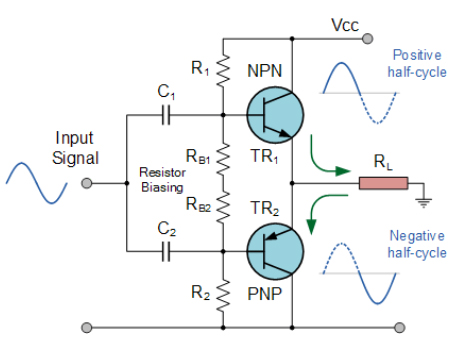
\includegraphics[weidth=10cm]{1.jpg} 
 
\end{flushleft}
\begin{flushleft}
Los amplificadores Push-Pull utilizan dos transistores "complementarios" o coincidentes, uno de tipo NPN y el otro de tipo PNP con ambos transistores de potencia que reciben la misma señal de entrada que es igual en magnitud, pero en fase opuesta entre sí . Esto resulta en un transistor solamente amplificar la mitad o 180 o del ciclo de forma de onda de entrada mientras que el otro transistor amplifica la otra mitad o restante 180 o del ciclo de forma de onda de entrada con las resultantes de “dos mitades” está poniendo juntos de nuevo en la salida terminal.

A continuación, el ángulo de conducción para este tipo de circuito amplificador sólo es 180 o o 50% de la señal de entrada. Este efecto de empujar y tirar de los semiciclos alternos por los transistores da a este tipo de circuito su divertido nombre "push-pull", pero en general se lo conoce como el amplificador de clase B, como se muestra a continuación.

\end{flushleft}
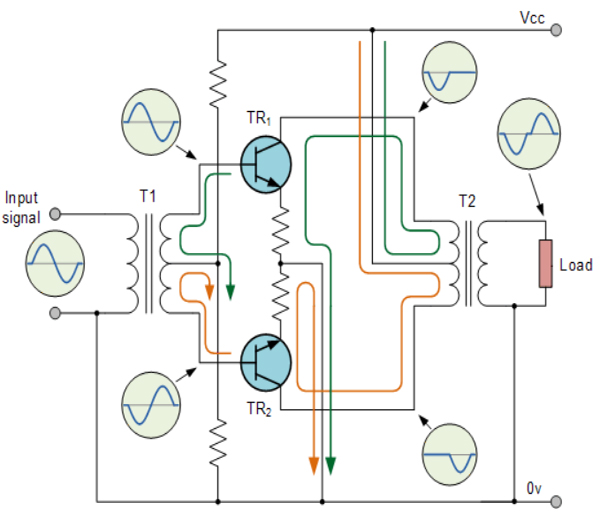
\includegraphics[weidth=10cm]{2.jpg} 
\begin{flushleft}
El circuito anterior muestra un circuito amplificador Clase B estándar que utiliza un transformador de entrada con toma central compensada, que divide la señal de forma de onda entrante en dos mitades iguales y que están desfasadas 180 ° entre sí. Otro transformador con toma central en la salida se utiliza para recombinar las dos señales que proporcionan la mayor potencia a la carga. Los transistores utilizados para este tipo de circuito amplificador push-pull de transformador son ambos transistores NPN con sus terminales de emisor conectados entre sí.

Aquí, la corriente de carga se comparte entre los dos dispositivos de transistor de potencia a medida que disminuye en un dispositivo y aumenta en el otro a lo largo del ciclo de señal, reduciendo el voltaje y la corriente de salida a cero. El resultado es que ambas mitades de la forma de onda de salida ahora oscilan desde cero hasta el doble de la corriente de reposo, reduciendo así la disipación. Esto tiene el efecto de casi duplicar la eficiencia del amplificador a alrededor del 70%.

\end{flushleft}
\begin{flushleft}
Cuando una señal de entrada está presente en el secundario del transformador controlador T1 , las entradas de la base del transistor están "antifásicas" entre sí como se muestra, por lo tanto, si la base TR1 es positiva y conduce el transistor a conducción pesada, su corriente de colector aumentará pero al mismo tiempo, la corriente de base de TR2 se volverá negativa en el corte y la corriente de colector de este transistor disminuirá en una cantidad igual y viceversa. Por lo tanto, las mitades negativas son amplificadas por un transistor y las mitades positivas por el otro transistor dando este efecto de contrafase.

A diferencia de la condición de CC, estas corrientes alternas son ADITIVAS, lo que resulta en que los dos semiciclos de salida se combinan para reformar la onda sinusoidal en el devanado primario de los transformadores de salida que aparece a lo largo de la carga.

El funcionamiento del amplificador de clase B tiene polarización CC cero ya que los transistores están polarizados en el corte, por lo que cada transistor solo conduce cuando la señal de entrada es mayor que la tensión del emisor base . Por lo tanto, en la entrada cero hay salida cero y no se consume energía. Esto significa que el punto Q real de un amplificador de Clase B está en la parte Vce de la línea de carga, como se muestra a continuación.

\end{flushleft}
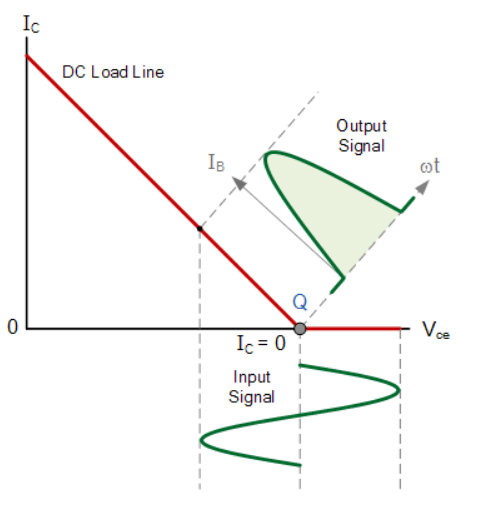
\includegraphics[width=10cm]{3.jpg} 
\begin{flushleft}
•
\end{flushleft}
\end{document}